% -*-coding: iso-latin-1  -*-
%---------------------------------------------------------------------
%
%                          Ap�ndice F
%
%---------------------------------------------------------------------

\chapter{Diagrama de clases final del proyecto}
	\label{ap1:classDiagra_vFinal}
		El presente documento puede ser consultado en el repositorio GitHub del proyecto\footnote{Acceso al material online: https://github.com/ERicBastida/BEcopter-Informe-Final/blob/master/Imagenes/DC\_BEcopter.png}.

%		\begin{figure}[h!]
%			\centering
%			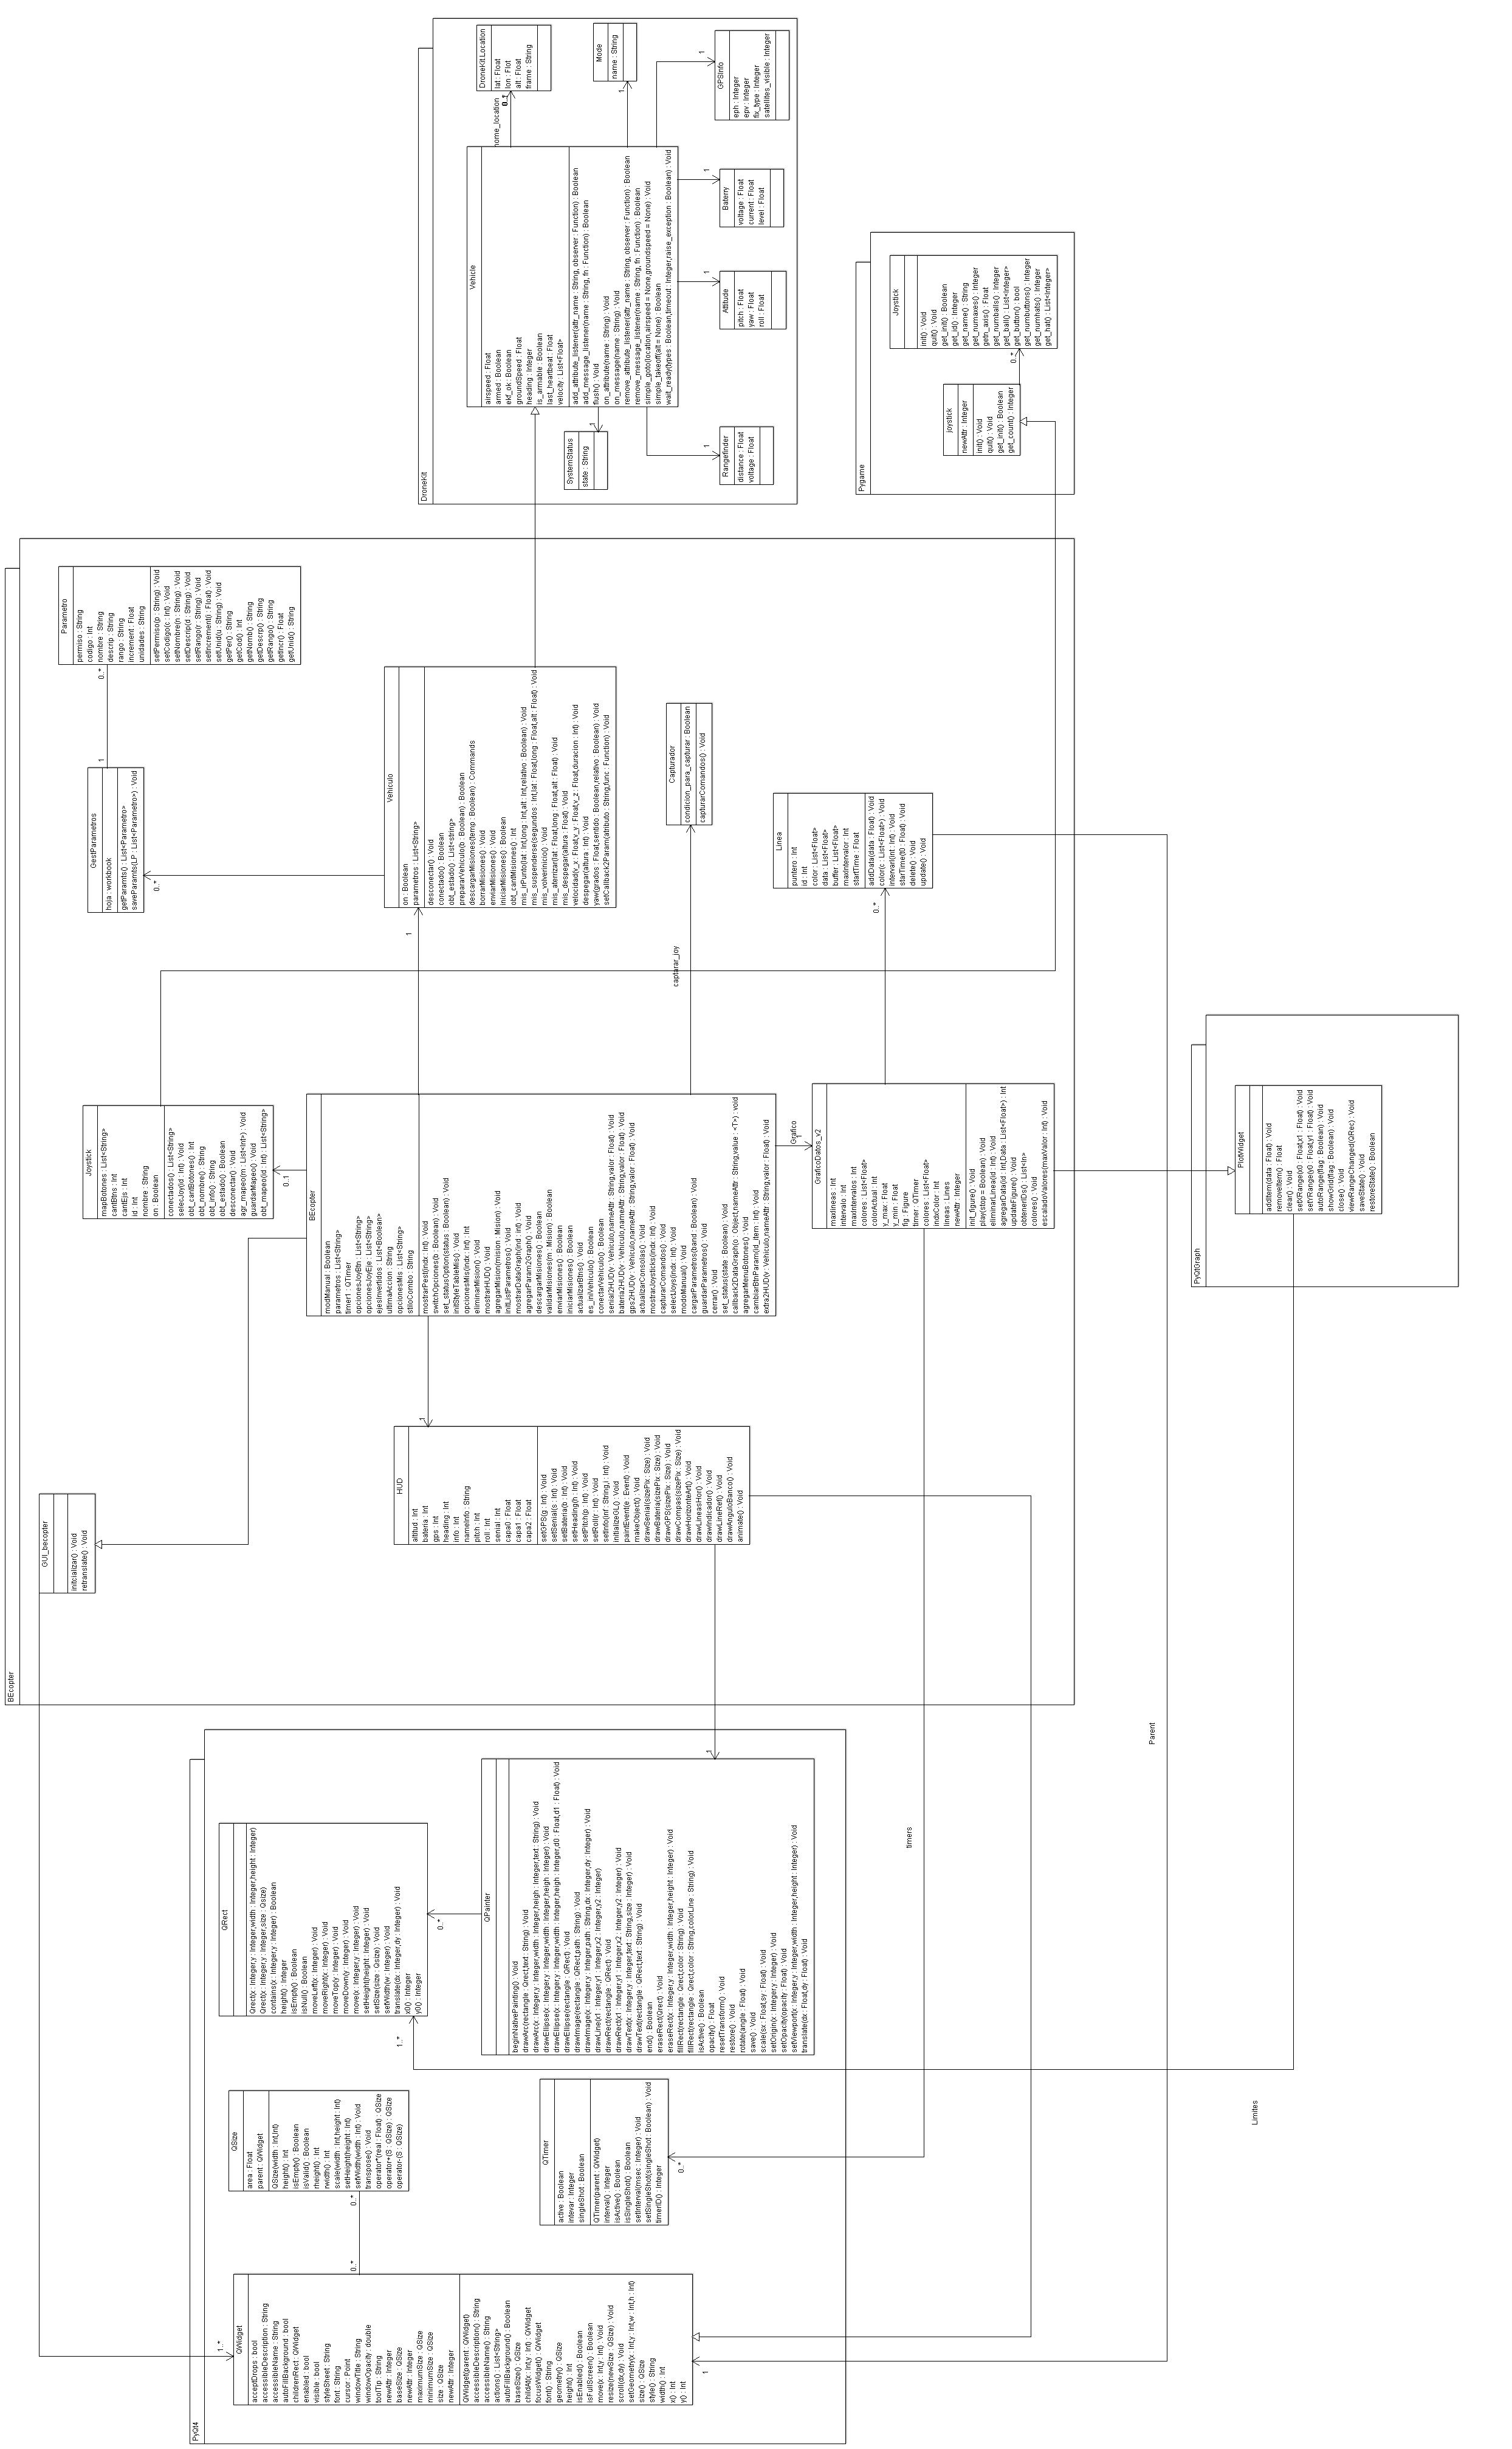
\includegraphics[width=\linewidth, height=0.93\textheight]{Apendices/Apendice_files/DC_vFinal}
%			\caption{Diagrama de clases v2, perteneciente al proyecto BEcoper.	}
%		\end{figure}







% Variable local para emacs, para  que encuentre el fichero maestro de
% compilaci�n y funcionen mejor algunas teclas r�pidas de AucTeX
%%%
%%% Local Variables:
%%% mode: latex
%%% TeX-master: "../Tesis.tex"
%%% End:
